\documentclass[ignoreonframetext,xcolor=table, unicode, 10pt]{beamer}
\geometry{paperwidth=140mm,paperheight=105mm}

\usepackage[utf8]{inputenc}
\usepackage[T1]{fontenc}
\usepackage[english,russian]{babel}
\usepackage{graphicx,pgf}
\usepackage{multimedia}
\usepackage{amsmath}
\usepackage{amssymb}
\usepackage{amsfonts}
\usepackage{mathtools}
\usepackage{scalerel}
\usepackage{tabularray}
\usepackage{colortbl}
\usepackage{nicematrix}
\usepackage{stackengine}
\usepackage{multirow}
\usepackage{supertabular}
\usepackage{multicol}
%\usepackage[oglav,spisok,boldsect,eqwhole,figwhole,hyperref,hyperprint,remarks,greekit]{fn2kursstyle}

\graphicspath{
	{./style/}
	{./illustr/}
	{./illustr/domain_rectangle_dirichlet_only/}
	{./illustr/domain_4/}
	{./illustr/domain_1_1/}
}

\usetheme{Warsaw}

\useinnertheme{circles}   %внутренняя тема
%\useoutertheme{smoothbars}   %внешняя тема
\usecolortheme{seahorse}     %цветовая схема
%\usefonttheme{serif}    %шрифты
%\defbeamertemplate*{footline}{shadow theme}
%\setbeameroption{hide notes}
\usepackage[document]{ragged2e}

%%Полужирный наклонный шрифт в формулах
\newcommand\be[1]{\text{\mathversion{bold}${#1}$}}
\newcommand\bi[1]{\text{\mathversion{bold}${#1}$}}
\newcommand\mathbi[1]{\text{\mathversion{bold}${#1}$}}
\newcommand\xrowht[2][0]{\addstackgap[.5\dimexpr#2\relax]{\vphantom{#1}}}

\renewcommand{\phi}{\varphi}
\newcommand\Tau{\scalerel*{\tau}{T}}
\renewcommand{\vec}[1]{\text{\mathversion{bold}${#1}$}}%{\bi{#1}}

%номера слайдов
\newcommand*\oldmacro{}%
\let\oldmacro\insertshorttitle%
\renewcommand*\insertshorttitle{%
	\oldmacro\hfill%
	\insertframenumber\,/\,\inserttotalframenumber}
\RequirePackage{caption}
\DeclareCaptionLabelSeparator{defffis}{ }
\captionsetup{justification=centering,labelsep=defffis}

%\title{Курсовая работа}
\title[Поиск потенциала электрического поля...]{Поиск потенциала электрического поля между заряженными пластинами}
\author[Егоров А.\,Д.]{Докладчик: Егоров А.\,Д.\and\\[0.5mm] Научный руководитель: Казаков К.\,Е.}

\institute[каф. Прикладная математика ФН-2]{Группа ФН2-62Б}
\date{\today}
\titlegraphic{
\includegraphics[width=2cm]{emblema.pdf}}
%\renewcommand{\vec}[1]{\text{\mathversion{bold}${#1}$}}

\begin{document}
	
	\begin{frame}[plain]
		\large
		\maketitle
		%\insertshortinstitute{Группа ФН2-62Б}
	\end{frame}

\begin{frame}{Постановка задачи}
	%\small
			
	\begin{block}{Задача}
		Найти потенциал электрического поля между двумя бесконечными пластинами, профиль одной из которых плоский, а профиль другой описывается некоторой периодической функцией. Значения потенциала на пластинах заданы и константны.	
	\end{block}
	\vspace*{-2.0mm}
	\begin{columns}\vspace*{-2.0mm}
		\column{0.45\textwidth}	
		\begin{block}{Математическая формулировка задачи}
		%	\vspace*{-5.0mm}
			\begin{equation*}
				\begin{cases}
					\Delta u (x, y)  = 0, \\
					u (x, y_a) = \phi_a, \\
					u (x, w(x)) = \phi_w, \\
					u (x, y) = u (x + T, y).\\
				\end{cases}
				\vspace*{0mm}
			\end{equation*} 
			$w(x)$ --- периодическая функция, задающая профиль искривленной пластины, $\phi_a, \phi_w$ --- значения потенциалов на пластинах.
		\end{block}
		\column{0.55\textwidth}	
			\centering
			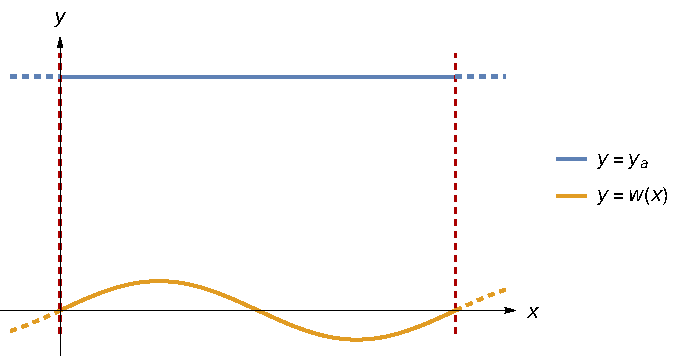
\includegraphics[width=1\textwidth]{illustr.pdf}
			\flushleft
			Иллюстрация области, в которой будет решаться задача
		
		
	\end{columns}
	
	\normalsize
\end{frame}

%\begin{frame}{Фильтрация исходных данных}
%		Необходимо отбросить следующие точки:
%		\begin{itemize}
	%		\item ошибки датчика (точки, значения в которых сильно отличаются от среднего значения на всем отрезке),
	%		\item залипания датчика (отрезки, на которых показания датчика неизменны, т.е. отличаются не более чем на $1 \%$).
%		\end{itemize}
%		\center
%		\includegraphics[width=1.\textwidth]{f_22608_10.08.28_data_raw_filtered_comparison.pdf}
	
%\end{frame}



\begin{frame}{Аппроксимация уравнения Лапласа}
	%\small
	%\begin{columns}
	%	\column{0.45\textwidth}
	%	\begin{block}{Уравнение Лапласа в двумерной области $\Omega \subset \mathbb{R}^2$}
	%		\begin{equation*}
	%			\begin{cases}
	%				- \Delta u  = 0 \ \  \text{в}\ \  \Omega, \\
	%				u = g \ \ \text{на}\ \  \Gamma_D,
	%			\end{cases}			
	%		\end{equation*}
	%		$\Gamma_D$ --- часть границы области, на которой заданы граничные условия первого рода, $\Gamma_D = \partial \Omega,$  $\Gamma_D \ne \emptyset$. 
	%	\end{block}
	%	\column{0.55\textwidth}
		
		Представим решение задачи в виде $u = u_0 + u_g,$
		где
		$u_0$ --- функция, обращающаяся в ноль на границе $\Gamma_D$,
		$u_g$ --- произвольная функция, значения которой совпадают с $g$ на границе области, $u_g |_{\Gamma_D} = g$.
		
		\begin{block}{Задача с однородными граничными условиями первого рода на $\Gamma_D$ относительно функции $u_0$}
			\begin{equation*}
				\begin{cases}
					- \Delta u  = \Delta u_g \ \  \text{в}\ \  \Omega, \\
					u_0 = 0 \ \ \text{на}\ \  \Gamma_D.
				\end{cases}			
			\end{equation*}
		\end{block}
		
		\hspace*{-2mm}
		%	\column{0.6\textheight}
		\begin{block}{Слабая постановка задачи для определения $u_0 \in V_D$}
			\begin{equation*}
				\int_{\Omega} \nabla u_0 \cdot \nabla v \, d\Omega = 
				- \int_{\Omega} \nabla u_g \cdot \nabla v \, d\Omega,
			\end{equation*}	
			\begin{equation*}
				\quad v \in V_D = \left\{ v \in V: \ v |_{\Gamma_D} = 0 \right\},
			\end{equation*}
			Пространство $V$ состоит из произвольных заданных в $\Omega$ функций, имеющих суммируемые с квадратом первые производные.
		\end{block}
		
		
	
	%\end{columns}
	
	\normalsize
\end{frame}

\begin{frame}{}
	%\small
	%\begin{columns}
		
		
	%	\column{0.68\textheight}
		\begin{block}{Аппроксимация методом конечных элементов}
			\begin{equation*}
				\int_{\Omega} \nabla u_{0,h} \cdot \nabla \phi_{i} \, d\Omega = 
				- \int_{\Omega} \nabla u_{g,h} \cdot \nabla \phi_{i} \, d\Omega, \quad i \in I. 
			\end{equation*}
			где $\phi_i$ --- функции, образующие базис в пространстве $V_h$ (конечномерное пространство аппроксимирующее V), $ i = \overline{1, N}$,\\
			$I$ --- множество идексов ф-ий $\phi_i$, образующих базис в пространстве 
			$V_{D,h} = V_h \cap V_D(\Omega)$, $\Gamma_D$. $M = |I| < N,\ |I| > 1.$
		\end{block}
		Представляя неизвестное решение в виде линейной комбинации базисных функций:		
		\vspace*{-5mm}
		\begin{equation*}
			u_{0,h} = \sum_{i \in I} u_{0,h,i} \phi_i, \quad 
			u_{g,h} = \sum_{i = 1}^{N} u_{g,h,i} \phi_i, 
		\end{equation*}		
		Получим СЛАУ для определения неизвестных коэффициентов $\left\{u_{0, h, i}\right\}$:
		\begin{equation*}
			A u_{0,h} = b,
			\label{SLE}
		\end{equation*}
		где $A = A_{M \times M}$ --- матрица жесткости, $b = b_{M \times 1}$,
		\begin{equation*}
			A_{ij} = \int_{\Omega} \nabla \phi_i \cdot \nabla \phi_j \, d\Omega,
			\ i, j\in I,
			\quad
			b_i = - \sum_{j=1}^{N} u_{g,h, j} \int_{\Omega} \nabla \phi_i  \cdot \nabla \phi_j \, d\Omega, \  i \in I.
		\end{equation*}
	\normalsize
\end{frame}



\begin{frame}{Триангуляция области}
	%\small
	Зададим правильную триангуляцию $\Tau$ области $\Omega$.
	
	Для отдельного треугольника $T \in \Tau$ c координатами вершин $P_i = (x_i, y_i),$ $i=\overline{1,3}$, базисные функции $\phi_i$, соответствующие этим вершинам, в $T$ продолжены линейно.
	\begin{equation*}
		\phi_i(x_j, y_j) = \delta_{ij}, \quad 
		\nabla \phi_{i}(x,y) = \dfrac{1}{2 |T|} 
		\begin{pmatrix}
			y_{i+1} - y_{i+2} \\
			x_{i+2} - x_{i+1} \\
		\end{pmatrix}, \ i,j = 1,2,3,
	\end{equation*}
	где $|T|$ --- площадь треугольника. Тогда формулы коэффициентов СЛАУ примут вид	
	\begin{equation*}
		A_{ij} = \sum_{T \in \Tau}\int_{T} \nabla \phi_i \cdot \nabla \phi_j \, d\Omega 
		= \sum_{T \in \Tau} \dfrac{1}{4 |T|} 
		\begin{pmatrix}
			y_{i+1} - y_{i+2}\\
			x_{i+2} - x_{i+1}\\
		\end{pmatrix}^T
		\begin{pmatrix}
			y_{j+1} - y_{j+2}\\
			x_{j+2} - x_{j+1}\\
		\end{pmatrix},
		\  i, j\in I,
	\end{equation*}
	\begin{equation*}
		\begin{aligned}
			b_i = - \sum_{j=1}^{N} u_{g,h, j} & \sum_{T \in \Tau} \int_{T} \nabla \phi_i  \cdot \nabla \phi_j \, d\Omega = \\
			& = - \sum_{j=1}^{N} u_{g,h, j}  \sum_{T \in \Tau} \dfrac{1}{4 |T|} 
			\begin{pmatrix}
				y_{i+1} - y_{i+2}\\
				x_{i+2} - x_{i+1}\\
			\end{pmatrix}^T
			\begin{pmatrix}
				y_{j+1} - y_{j+2}\\
				x_{j+2} - x_{j+1}\\
			\end{pmatrix},
			\quad i \in I.
		\end{aligned}		
	\end{equation*}
	\normalsize
\end{frame}



\begin{frame}{Задача №\,1}%{Линейный сплайн}
	
	\begin{columns}
		\column{0.5\textwidth}
		
		Условие:
		\begin{equation*}
			\begin{cases}
				\Delta \varphi (x, y)  = 0, \\
				\varphi (x, 0) = \varphi (0, y) = \varphi (4, y) = 0, \\
				\varphi (x, 2) = 10.
			\end{cases}
		\end{equation*}
		
		\column{0.5\textwidth}\hspace*{-10mm}
		\centering
		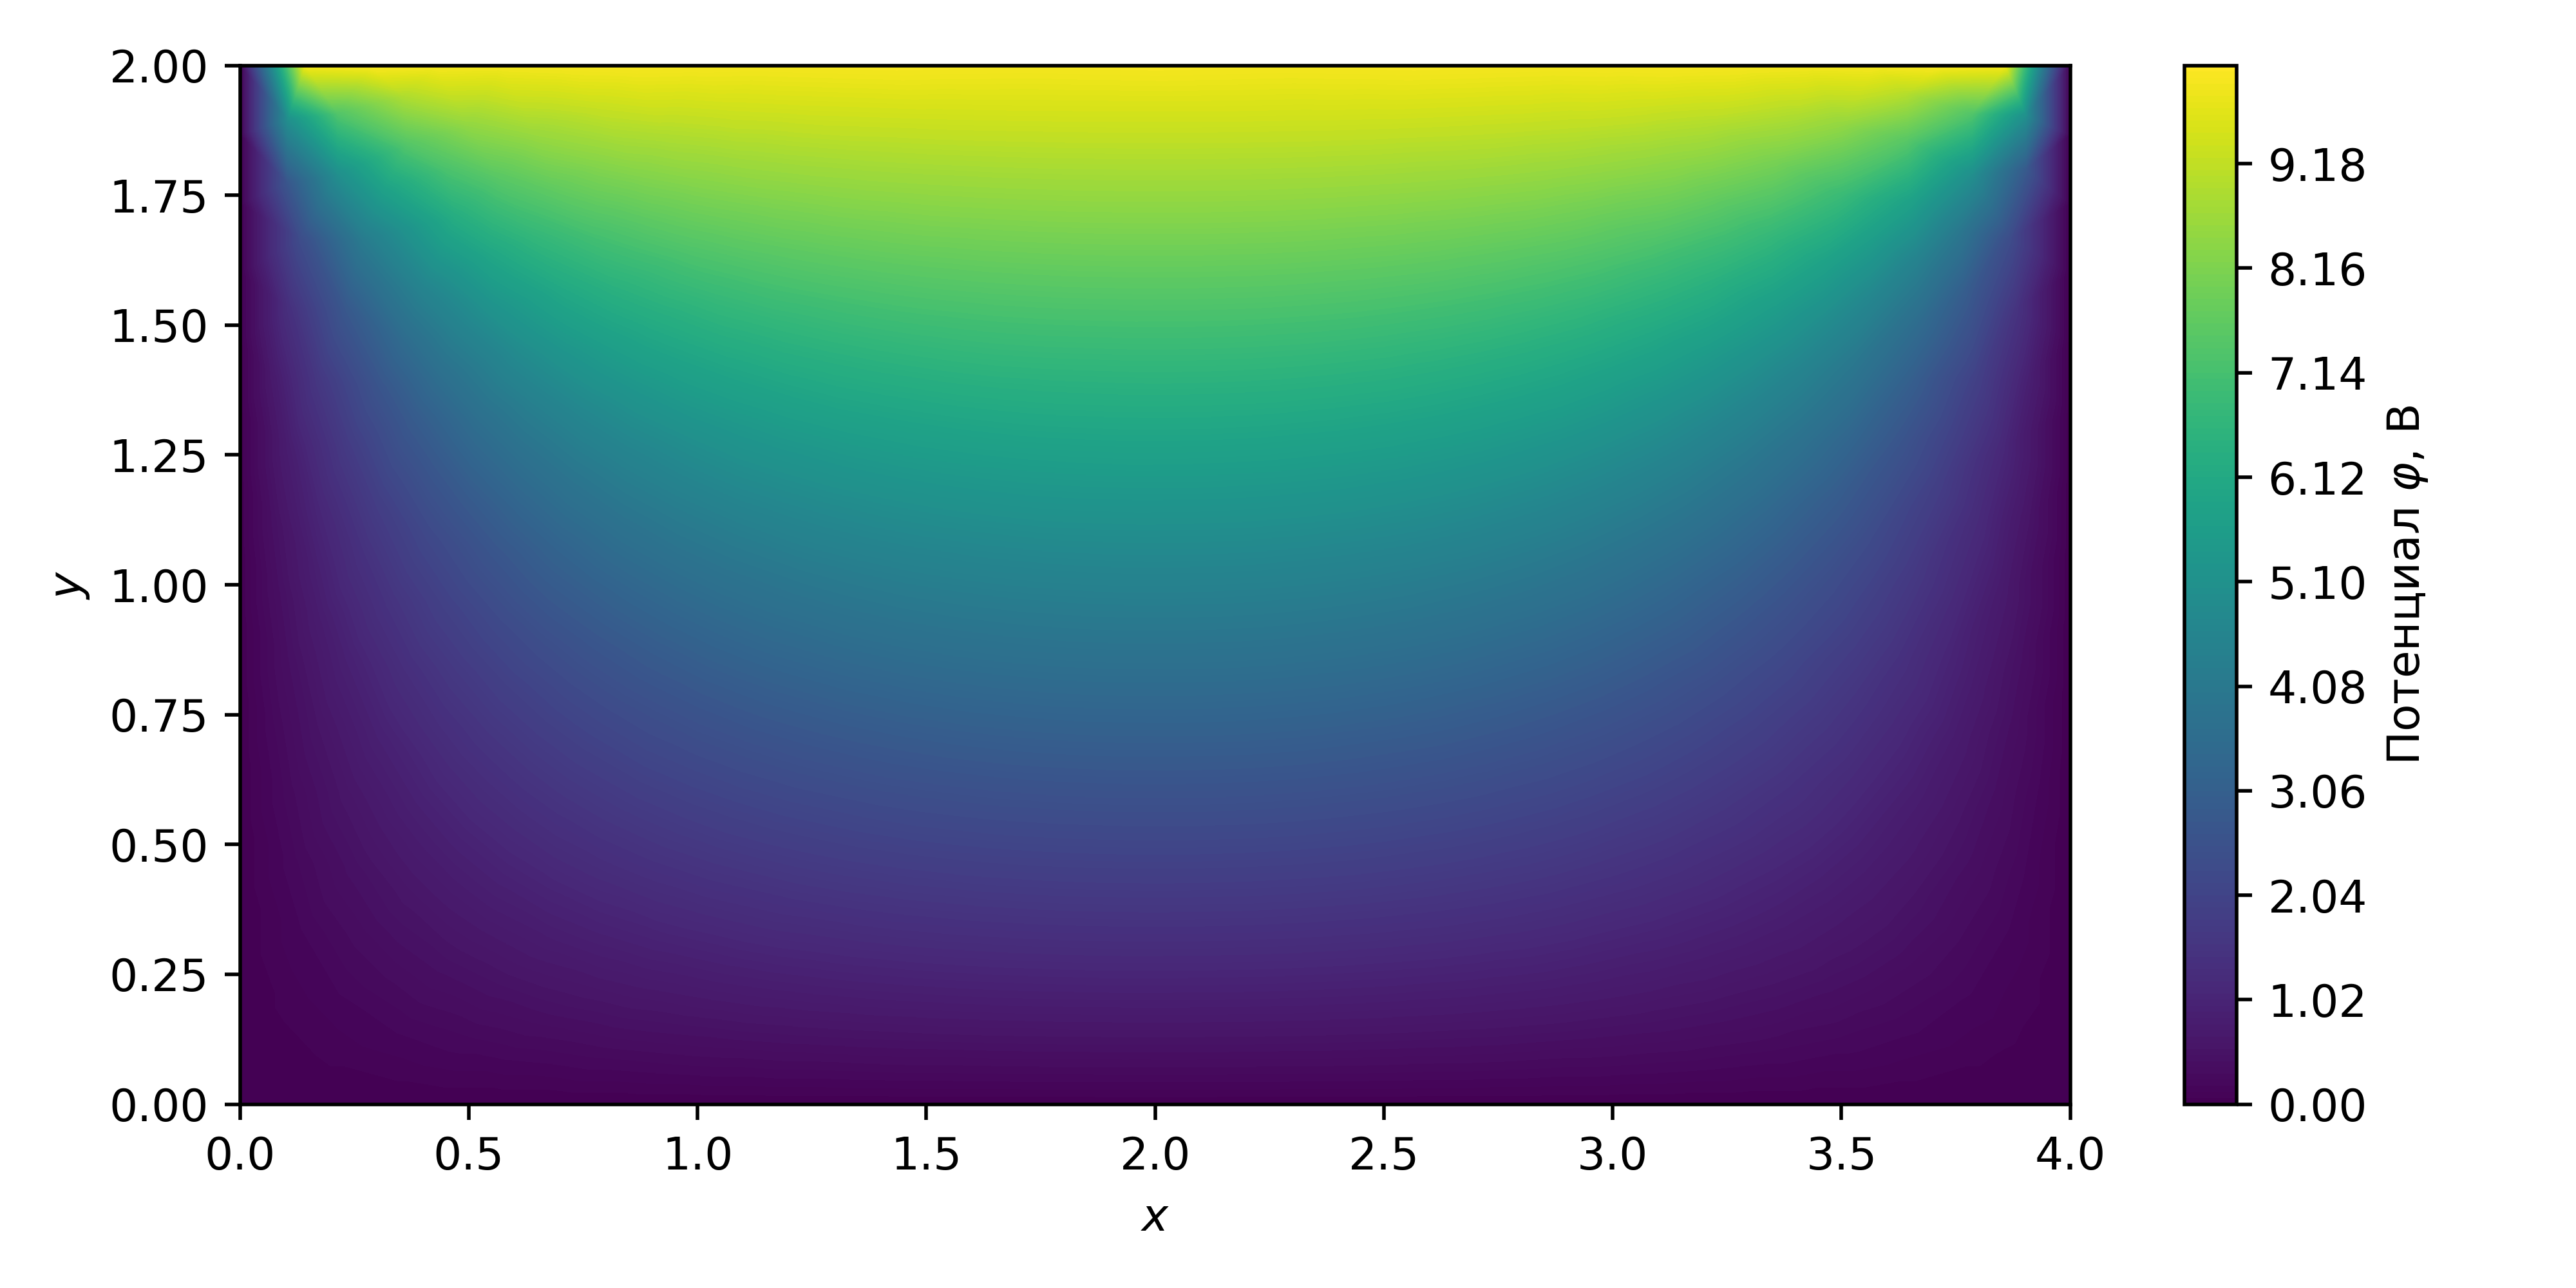
\includegraphics[width=1.2\columnwidth]{rect_dirichlet_only_exact_sol.png}
		
		\hspace*{-13mm}Точное решения\vspace*{2mm}
	\end{columns}
	
	\begin{columns}
		\column{0.5\textwidth}\hspace*{-5mm}
		\centering
		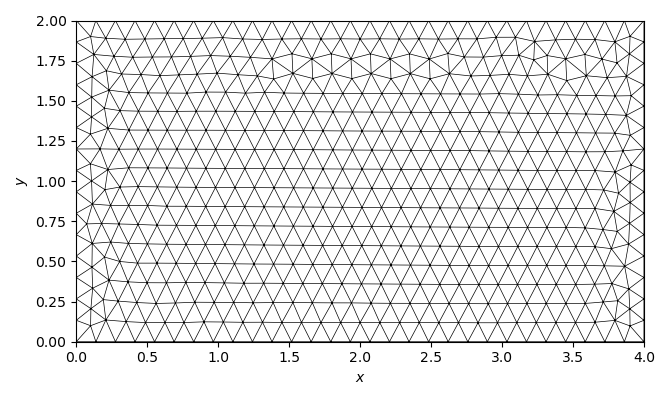
\includegraphics[width=1\columnwidth]{rect_dirichlet_only_001_calfem_net.png}\\ 
		Разбиение области $\Omega$ с элементы с $S_{max} = 0.01$
		
		\vspace*{-3.5mm}\column{0.5\textwidth}\hspace*{-10mm}
		\centering
		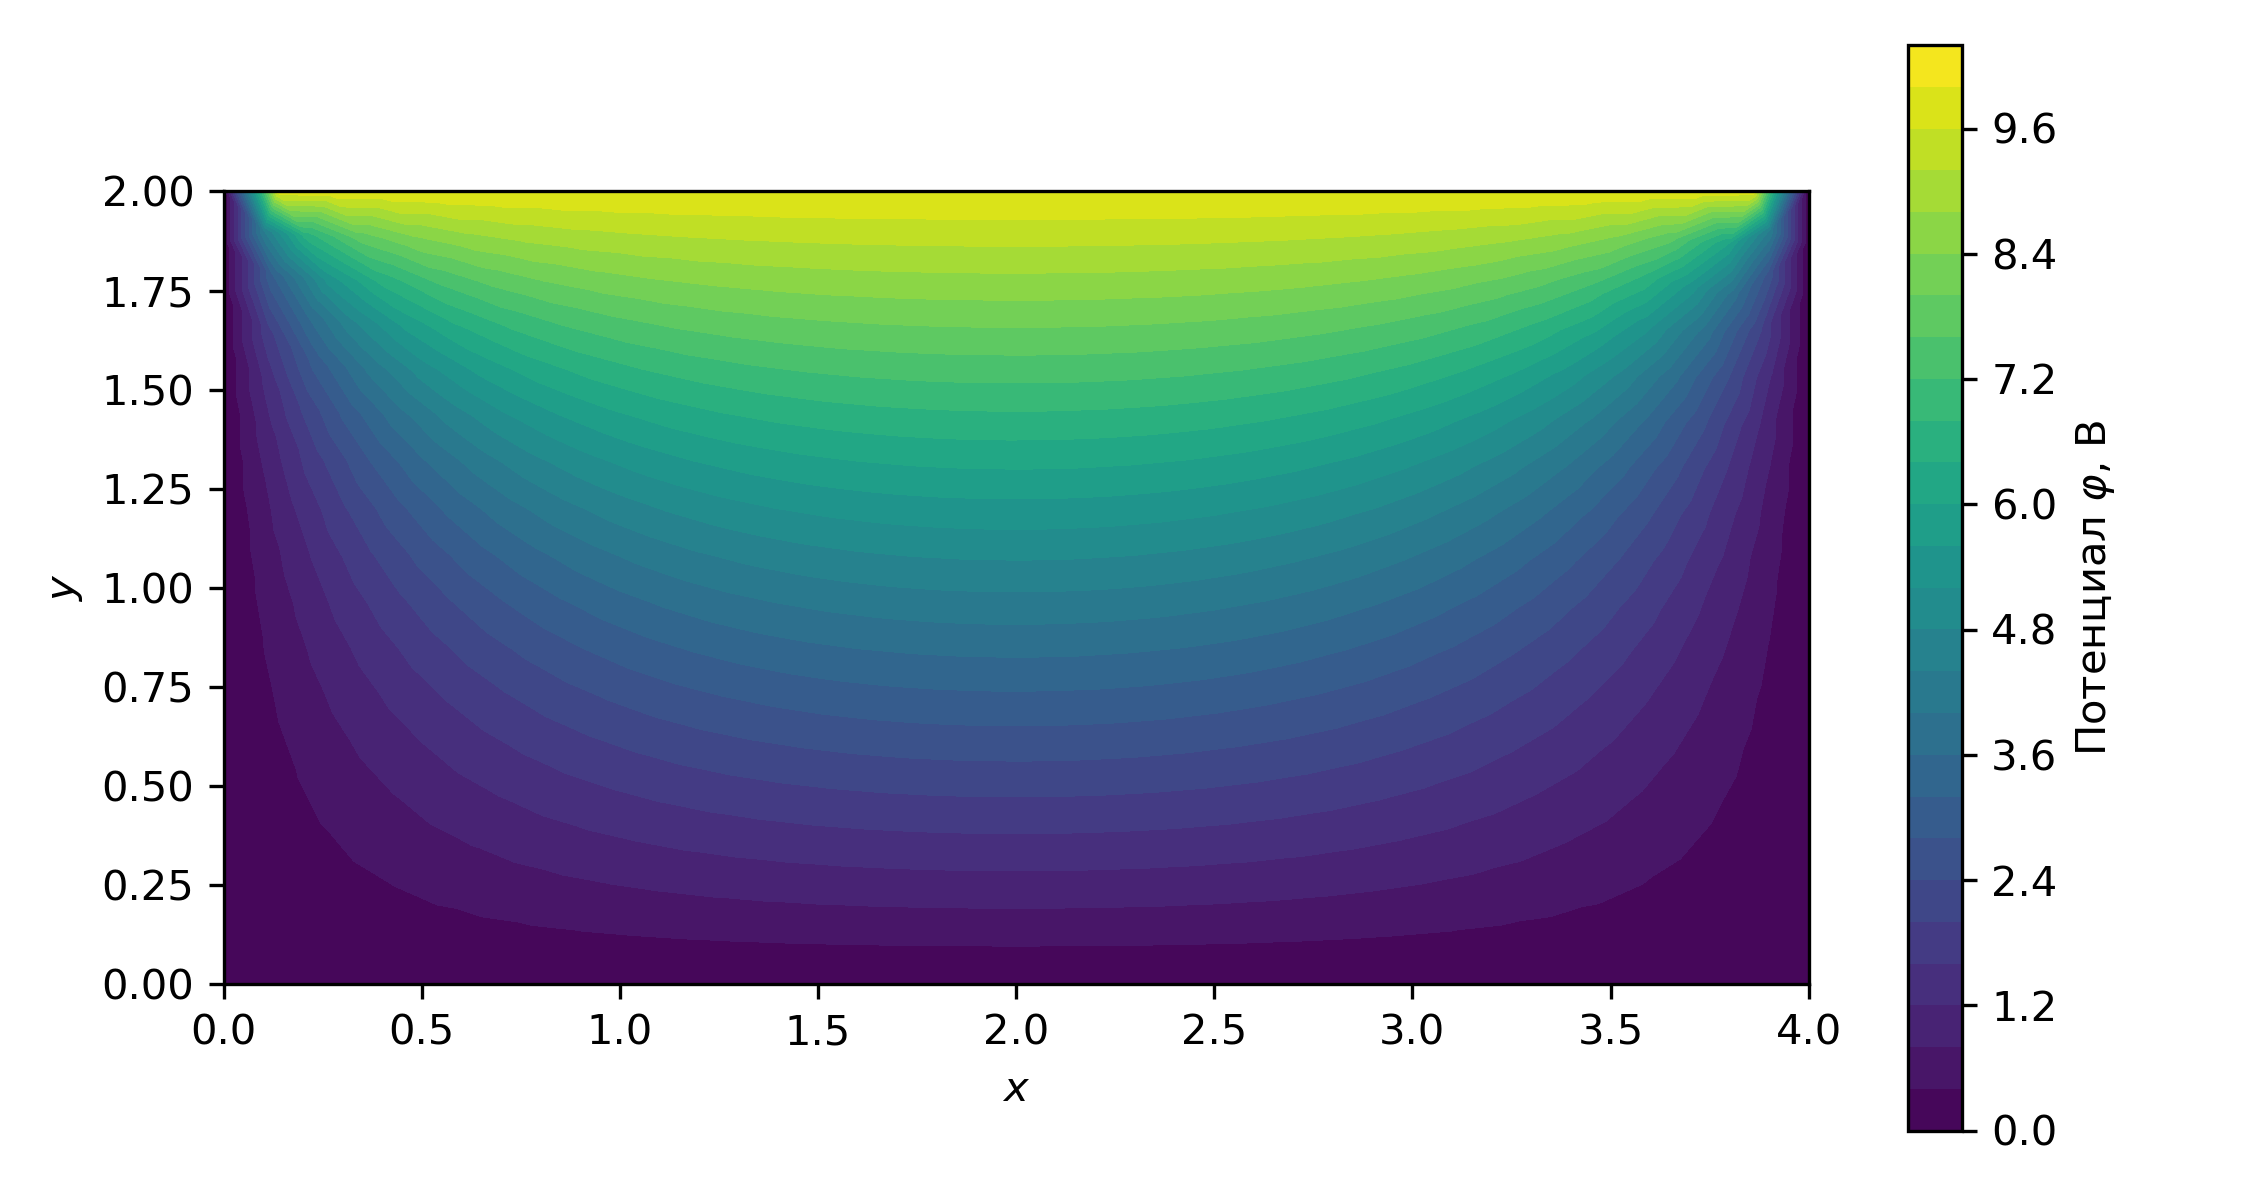
\includegraphics[width=1.2\columnwidth]{rect_dirichlet_only_001_calfem.png}\
		\hspace*{-13mm}Решение на сетке с $S_{max} = 0.01$
	\end{columns}
	
	%\begin{equation*}
	%	\displaystyle
	%	\varphi\left(x, y\right) = \sum_{n = 1}^{\infty} \dfrac{20 \left(1 - (-1)^n \right)}{\pi n \left[ \mathrm{exp}\left({-\dfrac{\pi n}{2}}\right) - \mathrm{exp}\left({\dfrac{\pi n}{2}}\right)  \right]} \left[ \mathrm{exp}\left({-\dfrac{\pi n}{4}} y \right) -  \mathrm{exp}\left({\dfrac{\pi n}{4}} y \right)  \right] \sin{\left( \dfrac{\pi n}{4} x \right)}
	%	\label{exact_solution}
	%\end{equation*}	
	
	
	\normalsize
	
\end{frame}

%\begin{frame}{}
	%
	%\begin{columns}
%		\column{0.5\textwidth}\hspace*{-5mm}
%		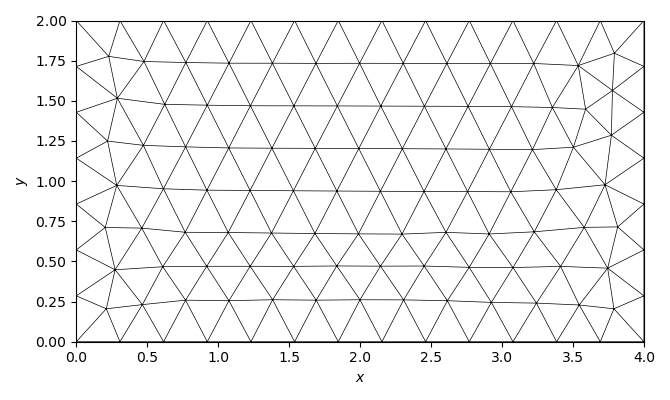
\includegraphics[width=1.\columnwidth]{rect_dirichlet_only_005_calfem_net.png}
%		Разбиение области $\Omega$ с элементы с $S_{max} = 0.05$
%		\column{0.5\textwidth}\hspace*{-10mm}
%		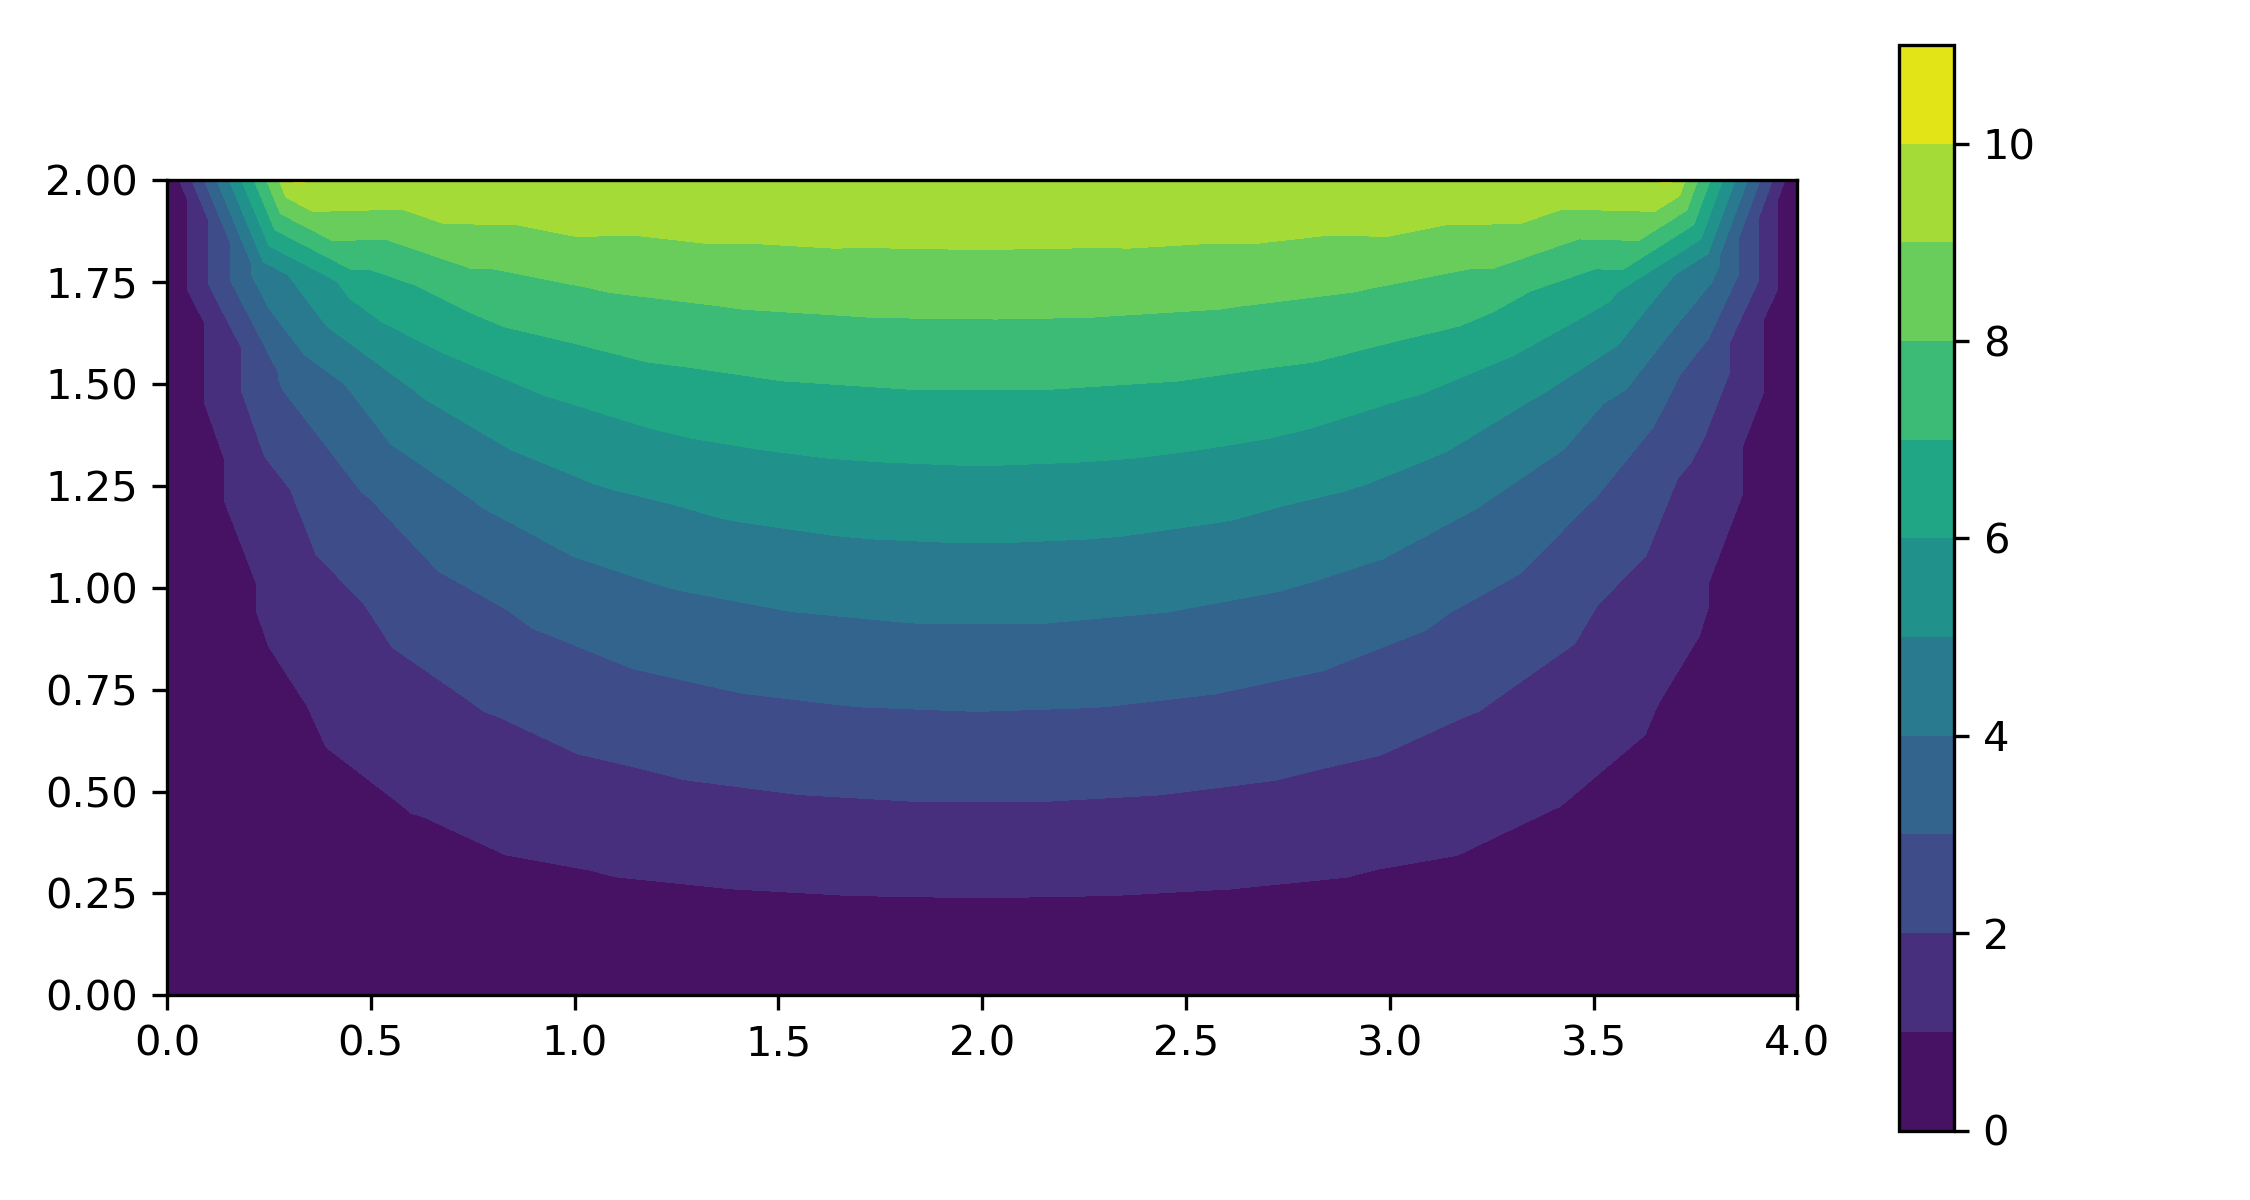
\includegraphics[width=1.2\columnwidth]{rect_dirichlet_only_005_calfem.png}
%		Решение на сетке с $S_{max} = 0.05$
%	\end{columns}
	%
%	\begin{columns}
%		\column{0.5\textwidth}\hspace*{-5mm}
%		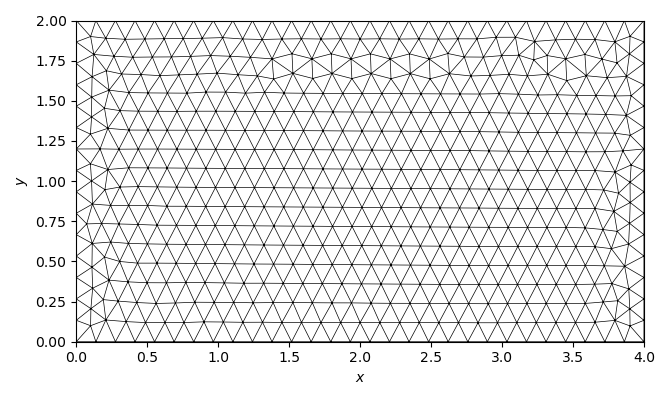
\includegraphics[width=1\columnwidth]{rect_dirichlet_only_001_calfem_net.png}\\ 
%		Разбиение области $\Omega$ с элементы с $S_{max} = 0.05$
%		
%		\column{0.5\textwidth}\hspace*{-10mm}
%		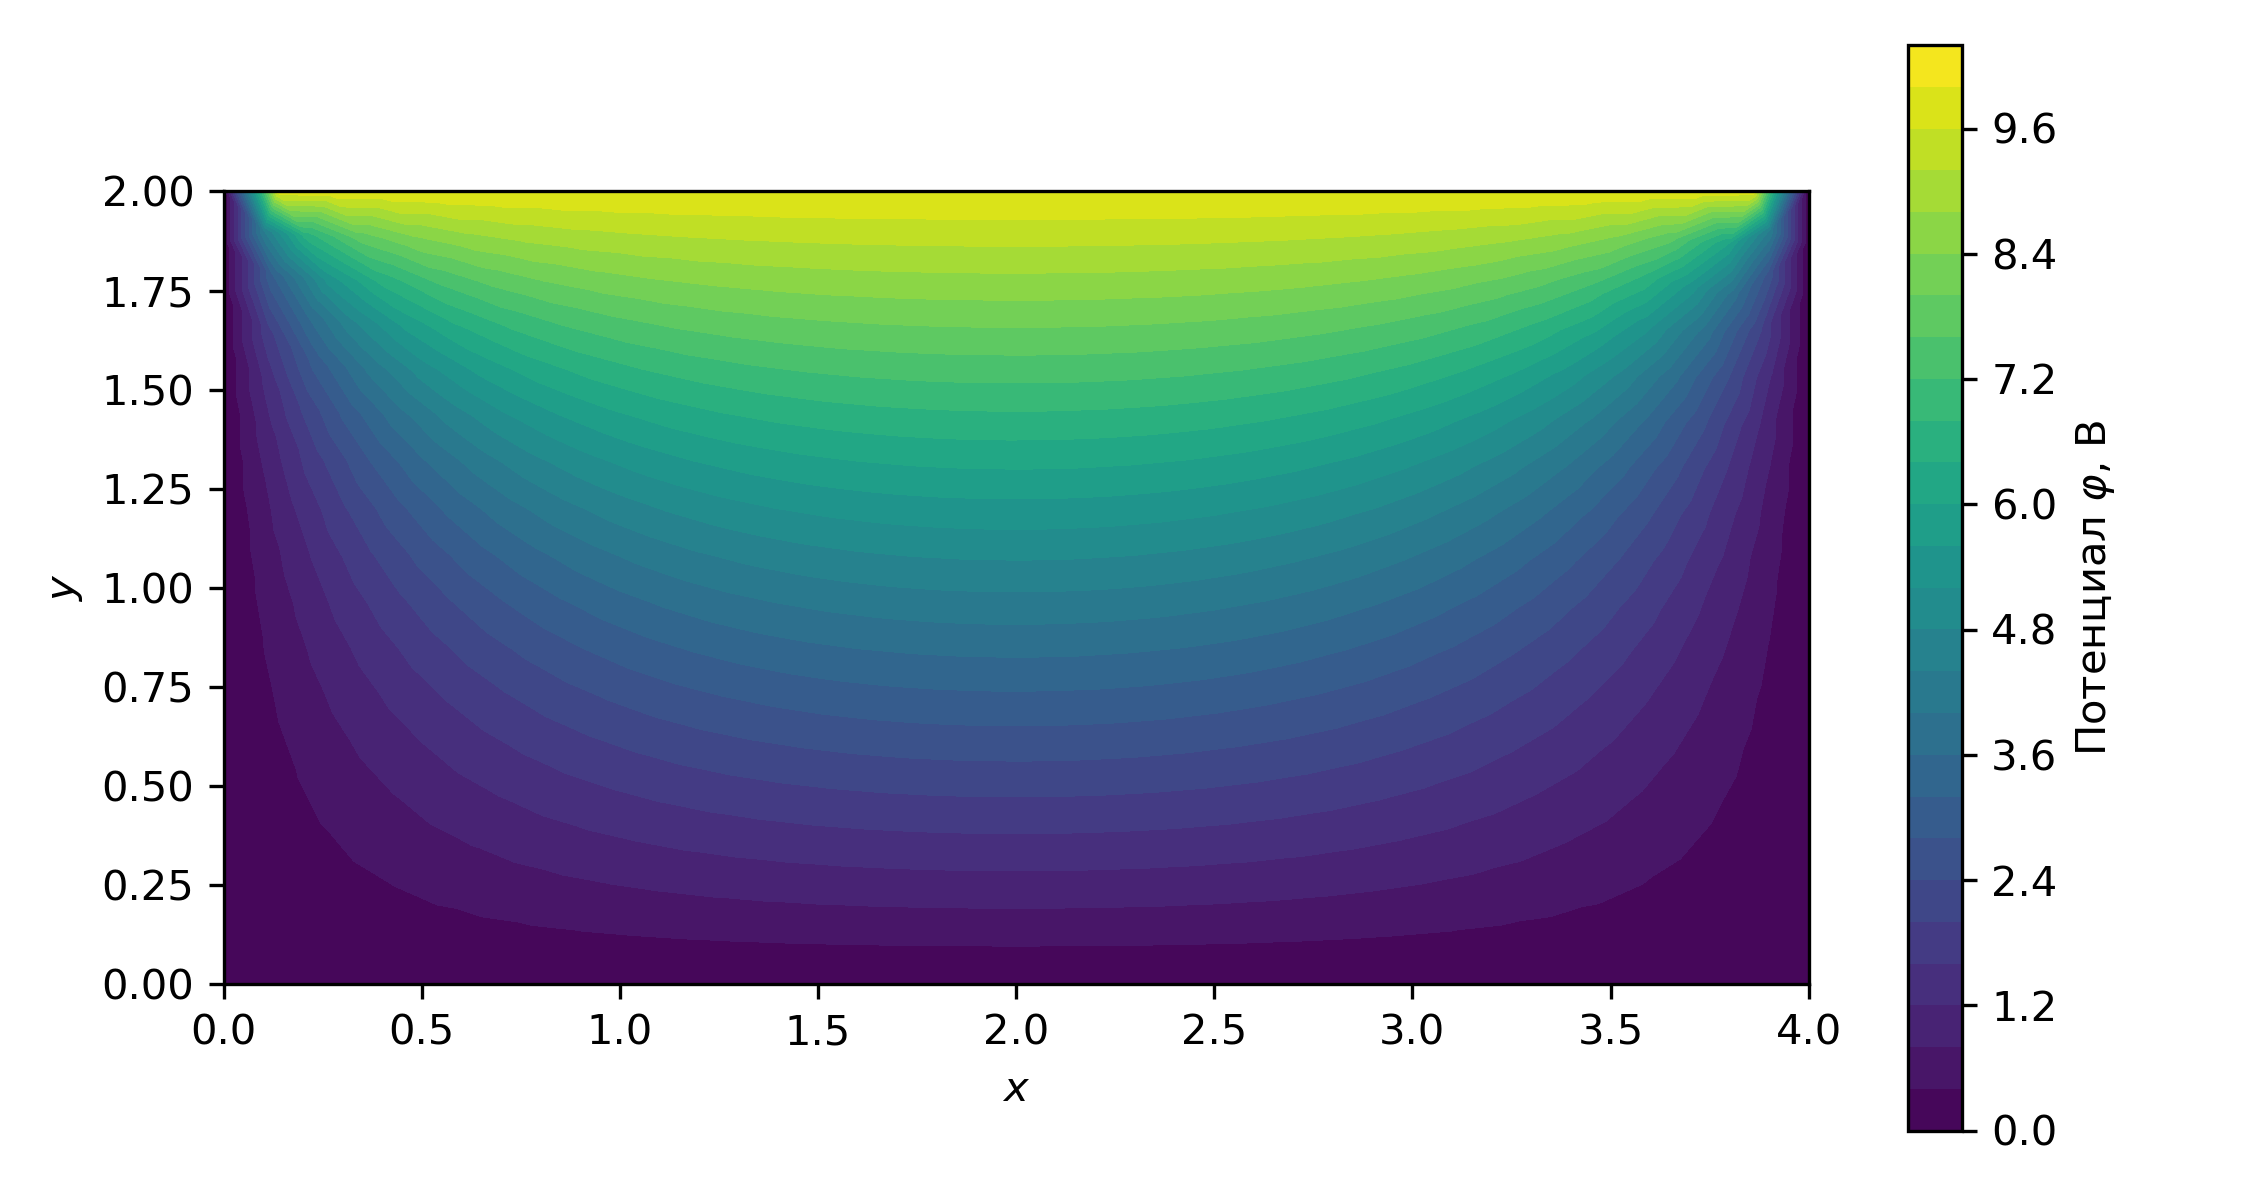
\includegraphics[width=1.2\columnwidth]{rect_dirichlet_only_001_calfem.png}\
%		Решение на сетке с $S_{max} = 0.01$
%	\end{columns}
	
	
%\end{frame}

\begin{frame}{}
	
	\begin{equation*}
		\mathrm{avg}(\mathrm{AbsErr}) = \dfrac{1}{N} \sum_{i = 1}^{N} \left| u_{exact, i} - u_{approx, i} \right|, \quad \text{$N$ --- количество узлов сетки}
	\end{equation*}
	\begin{equation*}
		\mathrm{Err}_{L_2}^2 = \| u_{exact} - u_{approx} \|_{L_2}^{2} \approx \sum_{i = 1}^{N_{el}} S_i
		\sum_{j = 1}^{3}  \dfrac{\phantom{|}(u_{exact,\,ij} - u_{approx,\,ij})^2}{3}.
		\label{l2_err_approx}
	\end{equation*}
	$N_{el}$ --- количество конечных элементов,
	$S_i$ --- площадь $i$-ого конечного элемента, $u_{exact,\,ij},\ u_{approx,\,ij}$ --- точное и приближенное значения решения в $j$-ом узле $i$-ого элемента.
	
	\normalsize
	\begin{table}[!h]
		\centering
		
		\vspace*{2mm}
		\begin{NiceTabular}{|c|c|c|c|c|}[hvlines,colortbl-like]
			
			\rowcolor[HTML]{CBCEFB}\xrowht{20pt}
			$N$
			& $S_{max}$
			& $\mathrm{avg}(\mathrm{h})$
			& $\mathrm{avg}(\mathrm{AbsErr})$
			& $\mathrm{Err}_{L_2}^2$  \\
			
			\rowcolor{white}\xrowht{7pt}
			216
			& 0.05
			& 0.3
			& 0.0289 
			& 0.0539 \\ 
			
			\rowcolor{white}\xrowht{7pt}
			1020
			& 0.01
			& 0.135
			& 0.0121
			& 0.0147 \\ 
			
			\rowcolor{white}\xrowht{7pt}
			1874
			& 0.005
			& 0.1
			& 0.0044
			& 0.0042 \\
			
			\rowcolor{white}\xrowht{7pt}
			10778
			& 0.001
			& 0.041
			& 0.00107
			& 0.00096 \\ 
			
			\rowcolor{white}\xrowht{7pt}
			22124
			& 0.0005
			& 0.029
			& 0.00053 
			& 0.00046 \\ 
			
		\end{NiceTabular}			
	\end{table}		

\end{frame}

\begin{frame}{}
	\small
	\vspace*{2mm}
	\begin{columns}
		\column{0.5\textwidth}
		\centering
		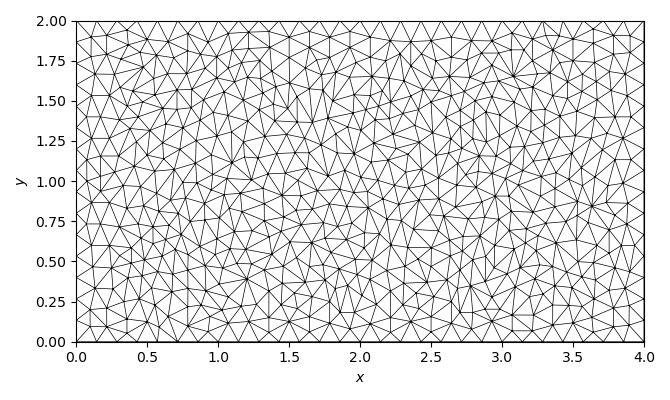
\includegraphics[width=1\columnwidth]{rect_dirichlet_only_001_net.png}\\ 
		\vspace*{-2mm}
		Разбиение области $\Omega$ с $S_{max} = 0.01$ и 
		$\mathrm{avg} \left( h_{max} / h_{min} \right) \approx 1.4 $
		
		\column{0.5\textwidth}
		\centering
		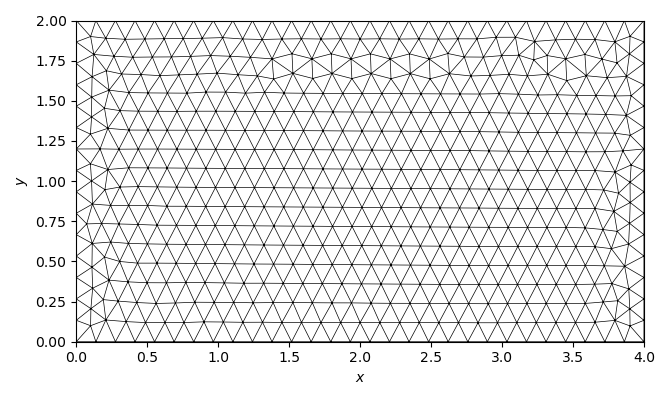
\includegraphics[width=1\columnwidth]{rect_dirichlet_only_001_calfem_net.png}
		\\
		\vspace*{-2mm}
		Разбиение области $\Omega$ с $S_{max} = 0.01$ и 
		$\mathrm{avg} \left( h_{max} / h_{min} \right) \approx 1.1$
	\end{columns}
	
	
	\normalsize
	\vspace*{0mm}
	\begin{table}
	\begin{NiceTabular}{|c|c|c|c|c|}[hvlines,colortbl-like]
		
		\rowcolor[HTML]{CBCEFB}\xrowht[()]{20pt}
		$\mathrm{avg}\left( h \right) $
		& $\mathrm{avg}\left( \dfrac{h_{max}}{h_{min}} \right) $
		& $\max \left( \dfrac{h_{max}}{h_{min}} \right) $
		& $\mathrm{avg}(\mathrm{AbsErr})$
		& $\mathrm{Err}_{L_2}^2$  \\
		
		
		0.3  \xrowht{7pt}
		&  1.1                                                                         
		& 1.5    
		& 0.03 
		& 0.05   \\
		
		0.3 \xrowht{7pt}
		&  1.4                                                                         
		& 2
		& 0.02 
		& 0.034  \\

		\rowcolor[HTML]{ECF4FF} \xrowht{7pt}
		0.135   
		& 1.1                                                                         
		&  1.4                                                                                        
		& 0.01                                                                                
		& 0.015  \\
		
		\rowcolor[HTML]{ECF4FF} \xrowht{7pt}
		0.127 
		&  1.4                                                                         
		&  2.3                                                                                        
		& 0.008                                                                               
		& 0.013  \\
		
		0.04 \xrowht{7pt}             
		&  1.1                                                                         
		&  1.4                                                                                        
		& 0.001                                                                               
		& 0.001  \\
		
		0.04 \xrowht{7pt}
		&  1.4                                                                         
		&  2.3                                                                                        
		& 0.003                                                                               
		& 0.007  \\

		\rowcolor[HTML]{ECF4FF} \xrowht{7pt}
		0.038          
		&  1
		&  1.5
		& 0.0007 
		& 0.0004 \\

		\rowcolor[HTML]{ECF4FF} \xrowht{7pt}
		0.036           
		&  1.4                                    
		&  2.3
		& 0.0052 
		& 0.0047    \\ 
		
	\end{NiceTabular}
	\end{table}

		
\end{frame}

\begin{frame}{Задача №\,2}
	\normalsize
	\vspace*{2mm}
	\begin{columns}[]
		\column{1\textwidth}
		Область $\Omega = \left\{ -\infty \leqslant x \leqslant \infty, \  w(x) \leqslant y \leqslant 2 \right\}$, $w(x)$ --- периодическая функция с периодом $T = 2$, $w(x) = |x - 1| + 1, \forall x \in \left[ 0, 2 \right]$, 
		потенциал на верхней пластине равен 0 В, на нижней --- 10 В.
	
	\end{columns}
	\vspace*{5mm}
	\begin{columns}[]
		\column{0.5\textwidth}
		\ \ \! Рассмотрим задачу при $x \in \left[ 0, 2 \right]$:
		
		\begin{equation*}\hspace*{-10mm}
			\begin{cases}
				\Delta \phi (x, y)  = 0, \\
				\phi (x, 2) = 0, \\
				\phi (x, w(x)) = 10, \\
				\phi (0, y) = \phi (2, y).\\
			\end{cases}
		\end{equation*}
		\vspace*{-2mm}
		\centering \hspace*{-10mm}
		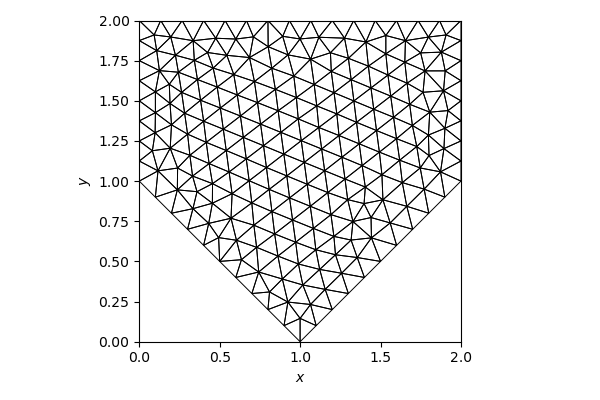
\includegraphics[width=1\columnwidth]{Test_domain_4_mesh001_calfem_net_1.png}\\
		\hspace*{-10mm} Разбиение $\Omega$ с $S_{max} = 0.01$
		
		\column{0.5\textwidth}
		\hspace*{-25mm}
		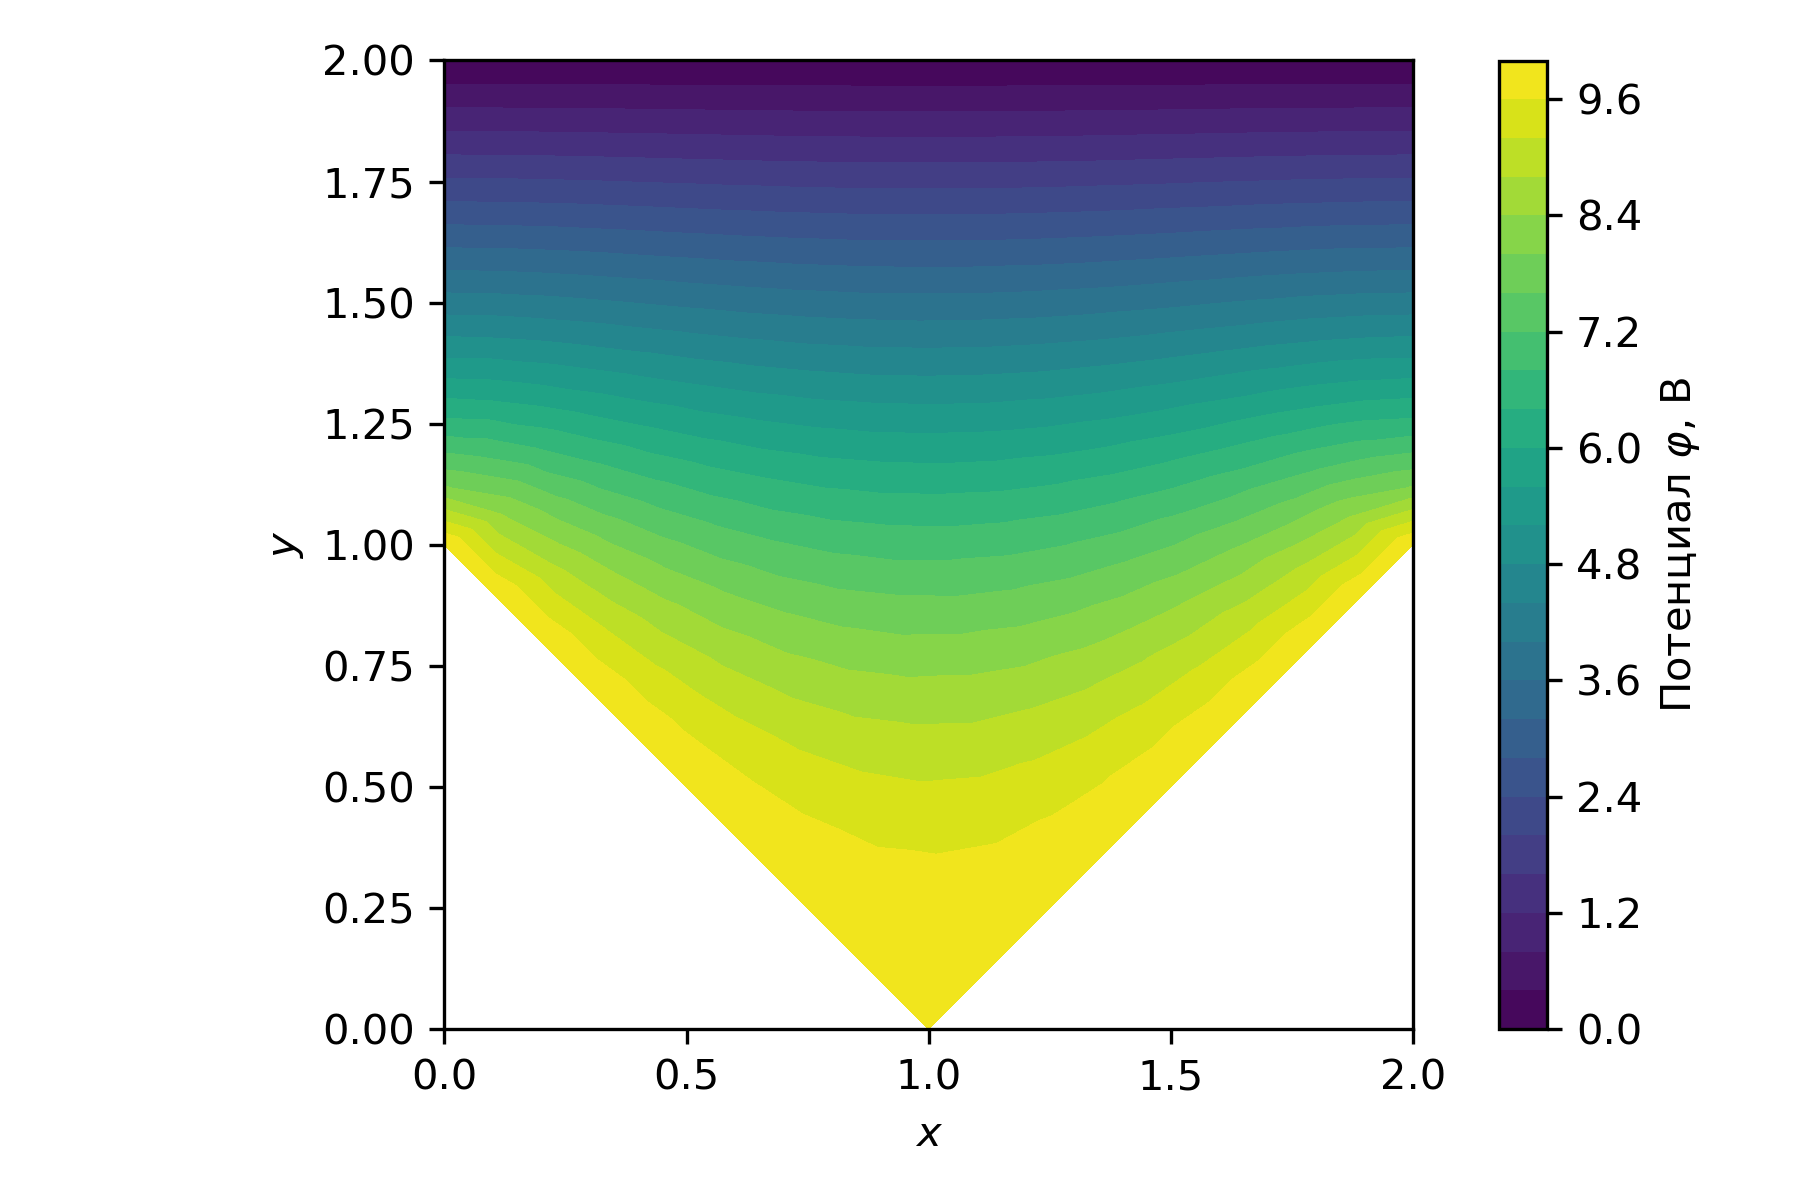
\includegraphics[width=1.5\columnwidth]{Test_domain_4_mesh001_calfem.png}\\
		Решение на сетке с $S_{max} = 0.01$
	\end{columns}
	
	
\end{frame}


\begin{frame}{}%{Оптимизированная сетка}
	\small
	\centering
	\vspace*{2mm}\hspace*{10mm}
	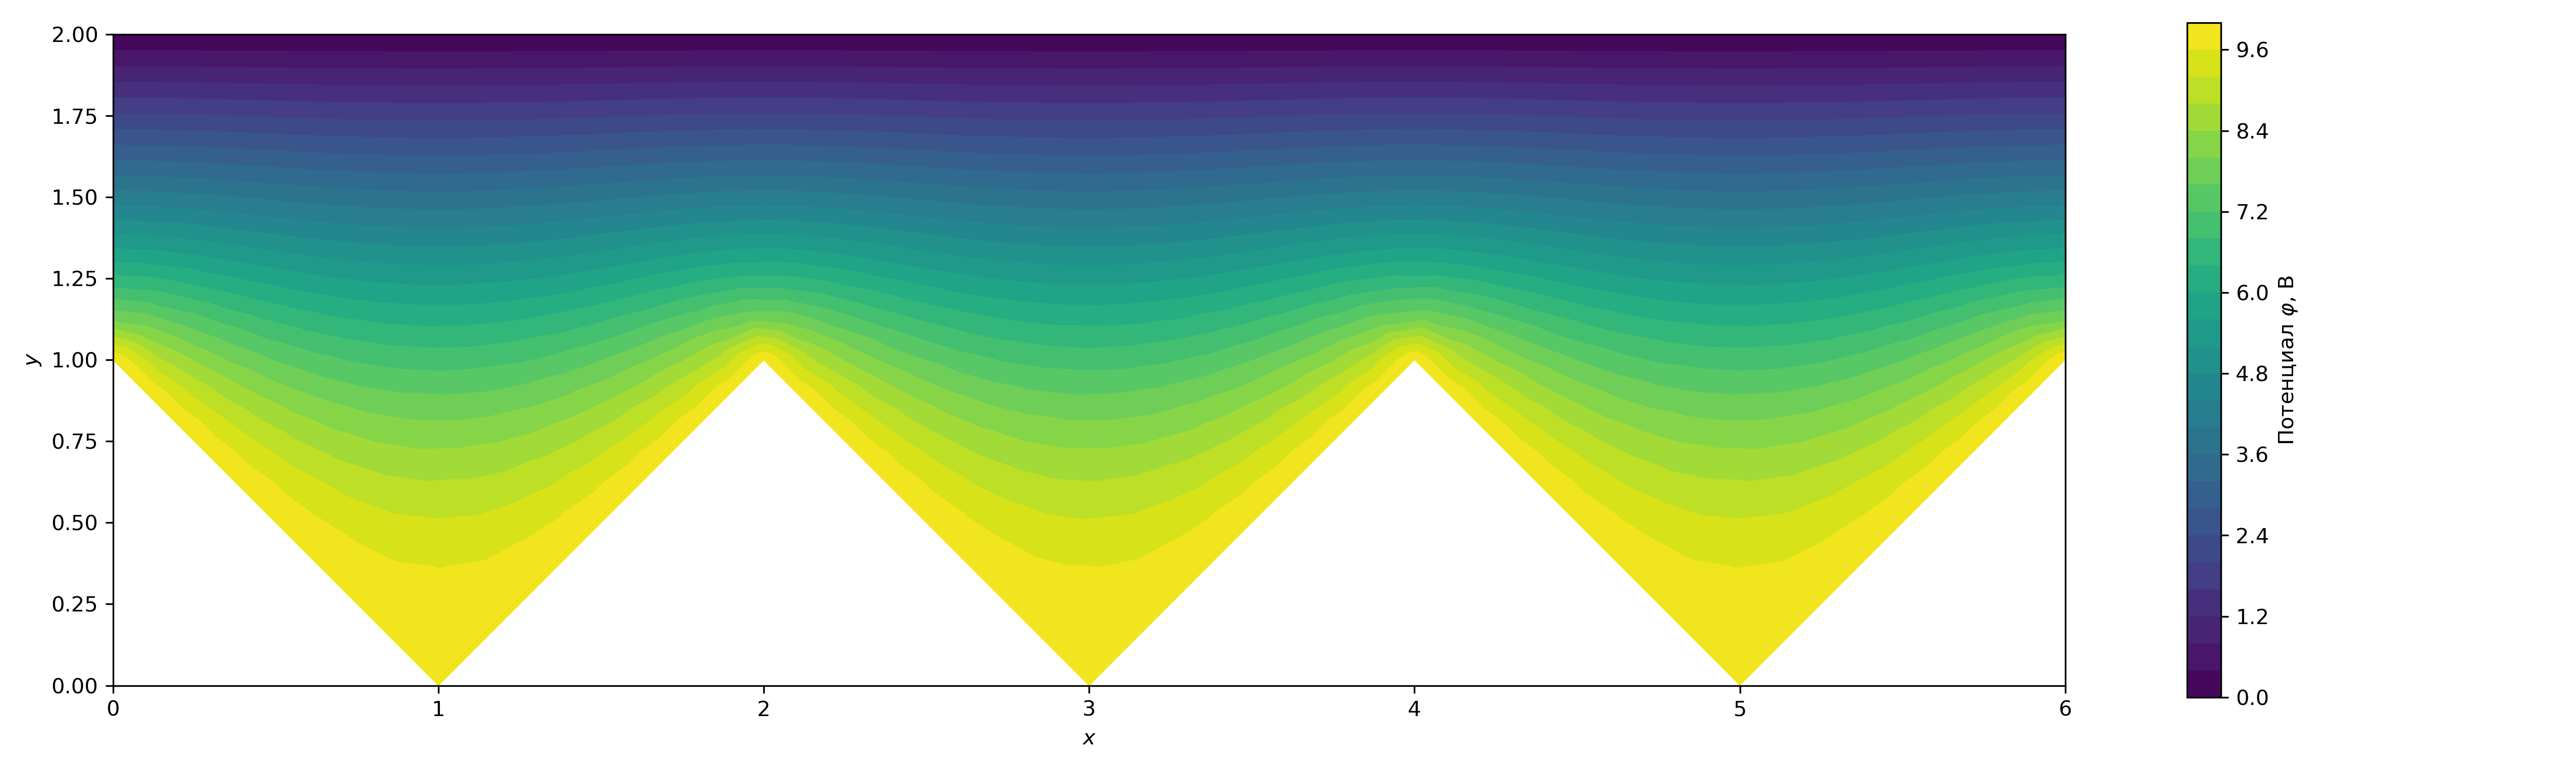
\includegraphics[width=0.9\textwidth]{Test_domain_4_mesh001_3_in_row_calfem.png}\\
	Решение на отрезке $\left[ 0, 6 \right]$ на сетке с $S_{max} = 0.01$ 
	
	\begin{table}[!h]
		\centering
		
		\vspace*{0mm}
		\begin{NiceTabular}{|c|c|c|}[colortbl-like]
			
			\hline
			\rowcolor[HTML]{CBCEFB}\xrowht{15pt}
			Область решения
			& Координаты $(x, y)$
			& Значение потенциала $\phi$, В\\
			
			\hline
			
			\multirow{2}{*}{1 период $w(x)$} \xrowht{5pt}
			& (0.0, 1.27)                                                      
			& 6.3158	\\ \cline{2-3} 
			
			\xrowht{5pt}
			& (2.0, 1.27)                                                      
			& 6.3158	\\ \hline
			
			\rowcolor[HTML]{ECF4FF}\xrowht{5pt}
			\multirow{4}{*}{3 периода $w(x)$} 
			& (0.0, 1.27)                                                     
			& 6.3093	\\ \cline{2-3}
			 
			\rowcolor[HTML]{ECF4FF}\xrowht{5pt}
			& (2.0, 1.27)                                                      
			& 6.2896	\\ \cline{2-3} 
			
			\rowcolor[HTML]{ECF4FF}\xrowht{5pt}
			& (4.0, 1.27)                                                      
			& 6.2946    \\ \cline{2-3} 
			
			\rowcolor[HTML]{ECF4FF}\xrowht{5pt}
			& (6.0, 1.27)                                                      
			& 6.3093	
			\\ 
			
			\hline
			
			\multirow{2}{*}{1 период $w(x)$} \xrowht{5pt} 
			& (0.0, 1.92)                                                      
			& 0.6551	\\ \cline{2-3}
			 
			\xrowht{5pt}
			& (2.0, 1.92)   
			& 0.6551	\\ 
			
			\hline
			
			\rowcolor[HTML]{ECF4FF}\xrowht{5pt}
			\multirow{4}{*}{3 периода $w(x)$} 
			& (0.0, 1.92)                                                      
			& 0.6547	\\ \cline{2-3} 
			\rowcolor[HTML]{ECF4FF}\xrowht{5pt}
			& (2.0, 1.92)                                                      
			& 0.6549	\\ \cline{2-3}  
			\rowcolor[HTML]{ECF4FF} \xrowht{5pt}     
			& (4.0, 1.92)                                                      
			& 0.6555	\\ \cline{2-3} 
			\rowcolor[HTML]{ECF4FF} \xrowht{5pt}         
			& (6.0, 1.92)                                                      
			& 0.6547 	\\ \hline
			
			
			
		\end{NiceTabular}
		
		
	\end{table}
	
\end{frame}

\begin{frame}{Задача №\,3}
	\normalsize
	\vspace*{2mm}
	\begin{columns}[]
		\column{1\textwidth}
		Область $\Omega = \left\{ -\infty \leqslant x \leqslant \infty, \  w(x) \leqslant y \leqslant 2 \right\}$, $w(x) = \dfrac{1}{2} sin \left(\dfrac{\pi x}{2} \right)$,
		потенциал на верхней пластине равен $12$ В, на нижней --- $-7$ В.
		
	\end{columns}
	\vspace*{5mm}
	\begin{columns}[]
		\column{0.5\textwidth}
		\ \ \! Рассмотрим задачу при $x \in \left[ 1, 5 \right]$:
		
		\begin{equation*}\hspace*{-10mm}
			\begin{cases}
				\Delta \phi (x, y)  = 0, \\
				\phi (x, 2) = 12, \\
				\phi (x, w(x)) = -7, \\
				\phi (1, y) = \phi (5, y).\\
			\end{cases}
		\end{equation*}
		\vspace*{-2mm}
		\centering \hspace*{-16mm}
		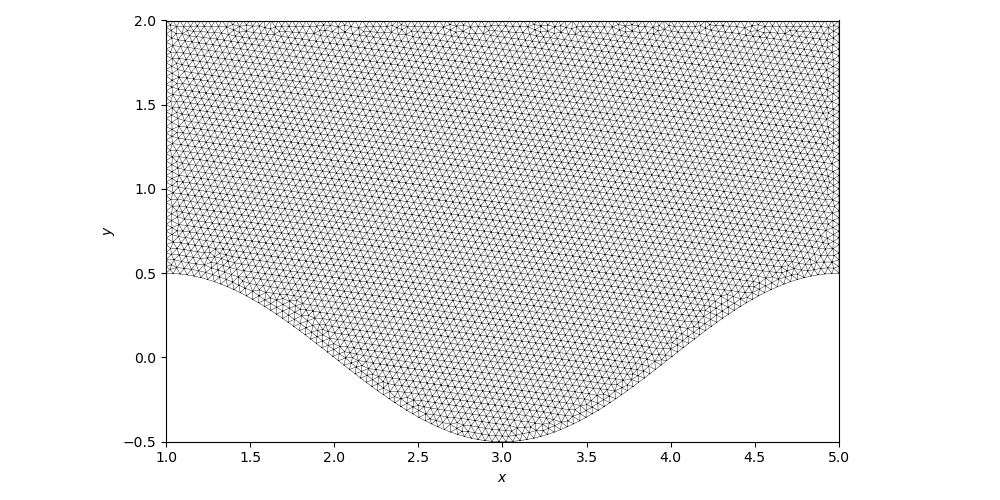
\includegraphics[width=1.1\columnwidth]{Test_domain_1_1_sin_mesh_0001_calfem_net_1.png}\\
		\hspace*{-14.5mm} Разбиение $\Omega$ с $S_{max} = 0.001$
		
		\column{0.5\textwidth}
		\hspace*{-22mm}
		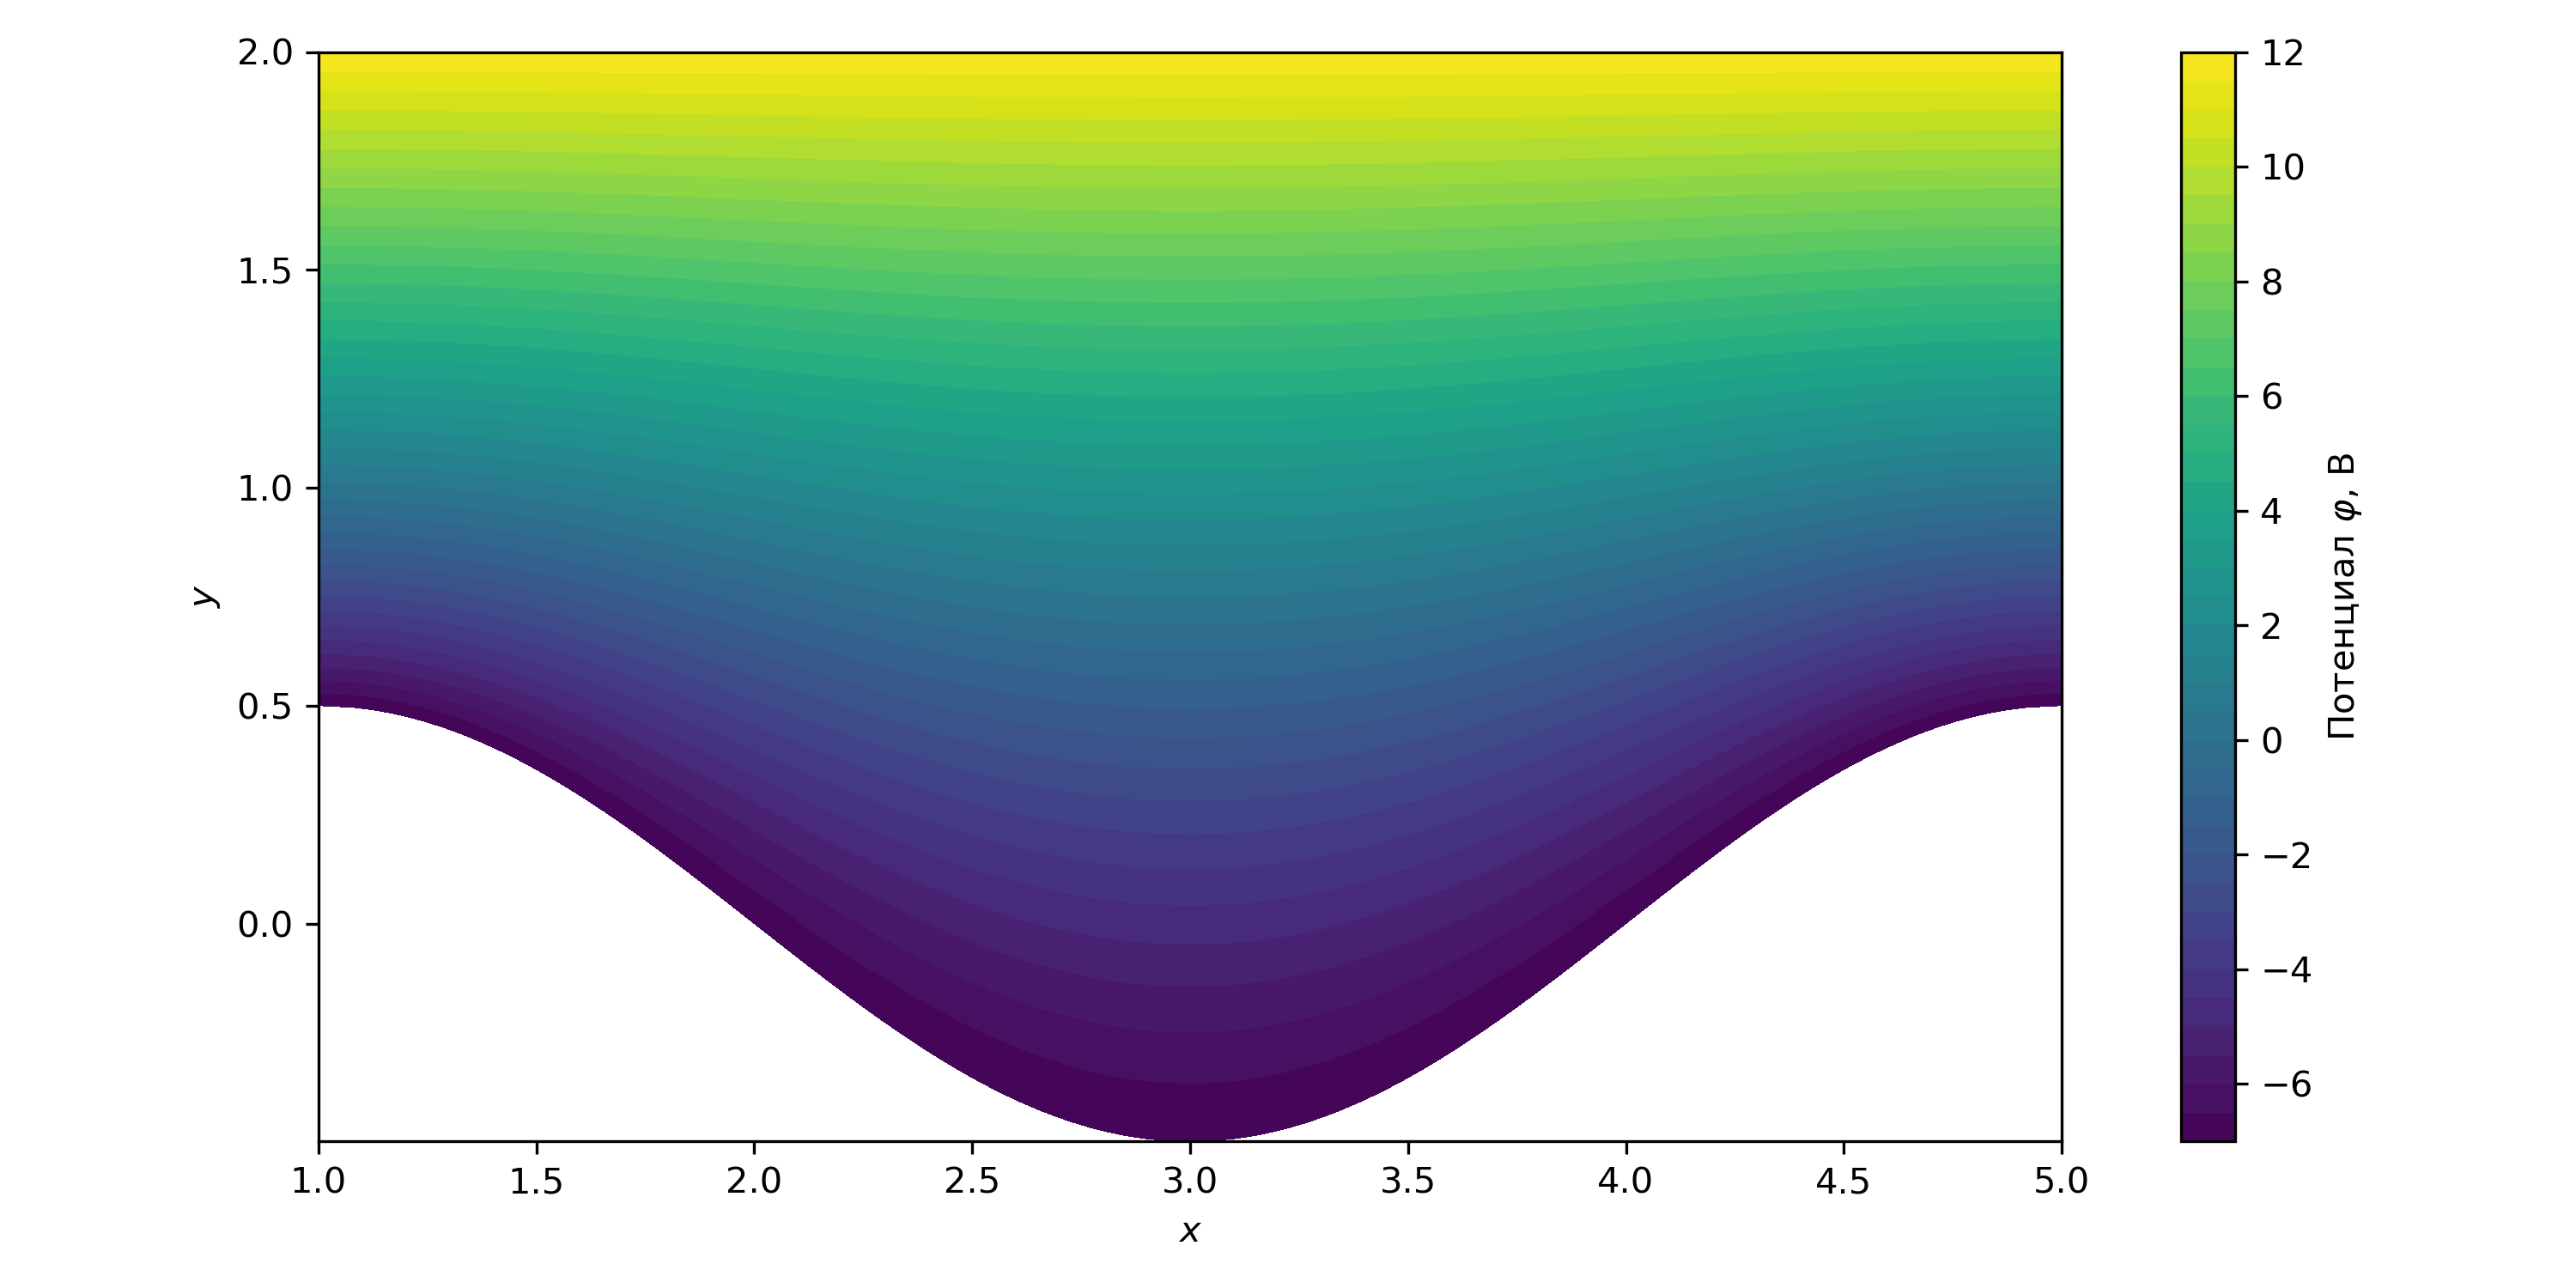
\includegraphics[width=1.5\columnwidth]{Test_domain_1_1_sin_mesh_0001_calfem.png}\\
		\hspace*{-3.5mm}Решение на сетке с $S_{max} = 0.001$
	\end{columns}
	
	
\end{frame}

\begin{frame}{}%{Оптимизированная сетка}
	\small
	
	\centering
	\vspace*{2mm}\hspace*{10mm}
	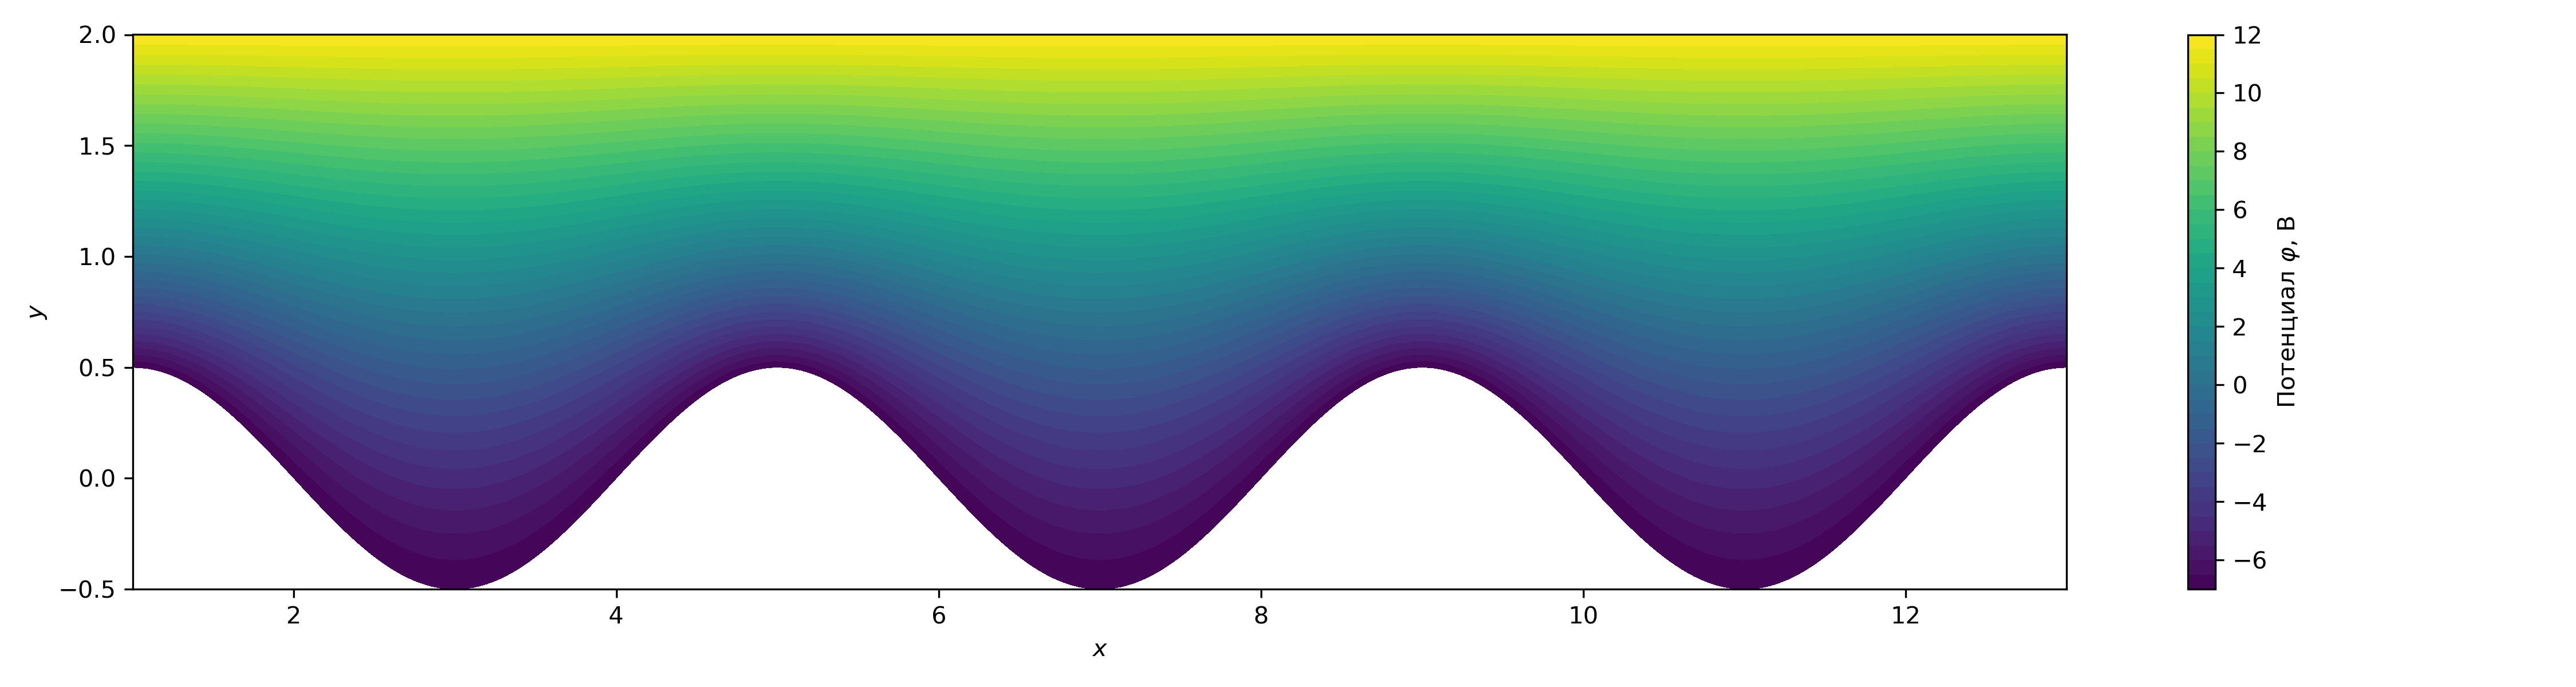
\includegraphics[width=0.9\textwidth]{Test_domain_1_1_sin_mesh_0001_3_in_row_calfem.png}\\
	Решение на отрезке $\left[ 1, 13 \right]$ на сетке с $S_{max} = 0.001$ 
	
	\begin{table}[!h]
		\centering
		
		\vspace*{0mm}
		\begin{NiceTabular}{|c|c|c|}[colortbl-like]
			
			\hline
			\rowcolor[HTML]{CBCEFB}\xrowht{15pt}
			Область решения
			& Координаты $(x, y)$
			& Значение потенциала $\phi$, В\\ 
			
			\hline
			
			\multirow{2}{*}{1 период $w(x)$}  
			& (1.0, 1.25)             
			& 3.4191          \\ 
			\cline{2-3} 
			
			& (5.0, 1.25)             
			& 3.4191          \\ 
			
			\hline
			
			\rowcolor[HTML]{ECF4FF} \xrowht{5pt} 
			\multirow{4}{*}{3 периода $w(x)$} 
			& (1.0, 1.25)             
			& 3.4191          \\ 
			\cline{2-3} 
			
			\rowcolor[HTML]{ECF4FF} \xrowht{5pt} 
			& (5.0, 1.25)             
			& 3.4185          \\ \cline{2-3} 
			
			\rowcolor[HTML]{ECF4FF} \xrowht{5pt} 
			& (9.0, 1.25)             
			& 3.4184          \\ \cline{2-3}
			 
			\rowcolor[HTML]{ECF4FF} \xrowht{5pt} 
			& (13.0, 1.25)            
			& 3.4191          \\ 
			
			\hline
			
			\multirow{2}{*}{1 период $w(x)$}  
			& (1.0, 1.6)            
			& 7.4927          \\ 
			\cline{2-3} 
			
			& (5.0, 1.6)             
			& 7.4927          \\ 
			\hline
			
			\rowcolor[HTML]{ECF4FF} \xrowht{5pt} 
			\multirow{4}{*}{3 периода $w(x)$} 
			& (1.0, 1.6)             
			& 7.4927          \\ 
			\cline{2-3} 
			
			\rowcolor[HTML]{ECF4FF} \xrowht{5pt} 
			& (5.0, 1.6)             
			& 7.4926          \\ 
			\cline{2-3} 
			
			\rowcolor[HTML]{ECF4FF} \xrowht{5pt} 
			& (9.0, 1.6)             
			& 7.4927          \\ 
			\cline{2-3} 
			
			\rowcolor[HTML]{ECF4FF} \xrowht{5pt} 
			& (13.0, 1.6)            
			& 7.4927        \\ 
			\hline
			
			
		\end{NiceTabular}
		
		
	\end{table}
	
\end{frame}
%%%%%%%%%%%%%%%%%%%%%%%%%%%%%%%%%%%%%%%%%%




\begin{frame}{Заключение}{}
	\large
	В ходе курсовой работы был изучен и реализован метод конечных элементов для решения уравнения Лапласа. Реализация метода была проверена на тестовом примере с известным решением, также с ее помощью были решены и исследованы несколько вариантов исходной задачи с разными профилями пластин и заданными на них потенциалами.
	Все описанные подходы выполнены на языке C++ с демонстрацией результатов работы.		
	
\end{frame}

\end{document}